\documentclass{article}
\usepackage[utf8]{inputenc}

\usepackage{amsthm}
\usepackage{amsmath}
\usepackage{amssymb}
\usepackage{amsfonts}
\usepackage{graphicx}
\usepackage{tikz}
\usepackage{authblk}

% 习惯最小的题号用自定义的id命令直接打出来
\newcommand{\id}{\subsubsection*}
\newcommand{\fc}{\frac}

\usepackage{geometry}
% 纸张尺寸大小
% 也可以手动写 left, right, top, bottom 参数
\geometry{a4paper, scale = 0.9}
%\geometry{left = 2.54cm, right = 2.54cm, top = 3.17cm, bottom = 3.17cm}

\usepackage{indentfirst}
\renewcommand{\baselinestretch}{1.2}


%TODO: Title
\title{MA234 Homework 1}

%TODO: Author
\author{Duolei WANG, SID:12012727}
\affil{wangdl2020@mail.sustech.edu.cn}

%TODO: Date
\date{}


\begin{document}
\maketitle
\begin{enumerate}
\item Finished.

\item 
\begin{enumerate}
\item Considering
\[H(\mathrm{Appealing}) = - p(\mathrm{Yes})\log_2 p(\mathrm{Yes}) - p(\mathrm{No})\log_2 p(\mathrm{No}) = 1\]

\item Considering
\begin{align*}
H(\mathrm{Taste}) &= -p(\mathrm{Salty})\log_2p(\mathrm{Salty}) - p(\mathrm{Sweet})\log_2 p(\mathrm{Sweet}) - p(\mathrm{Sour})\log_2 p(\mathrm{Sweet})\\
&= - 0.3 \cdot \log_2(0.3) - 0.4 \cdot \log_2(0.4) - \log_3(0.3)\\
&= 2.15\\
\end{align*}

and
\[p({\mathrm{Salty}}) H(\mathrm{Appealing |Salty}) + p({\mathrm{Sweet}})H(\mathrm{Appealing |Sweet}) +p({\mathrm{Sour}}) H({\mathrm{Size | Sour}})\]

one can calculate it is \(0.4\).

Thus \(Gain = 1.75\).

\item Considering using the sklearn.tree, with criterion entropy to build a tree, we can get

\begin{figure}[!hb]
    \centering
    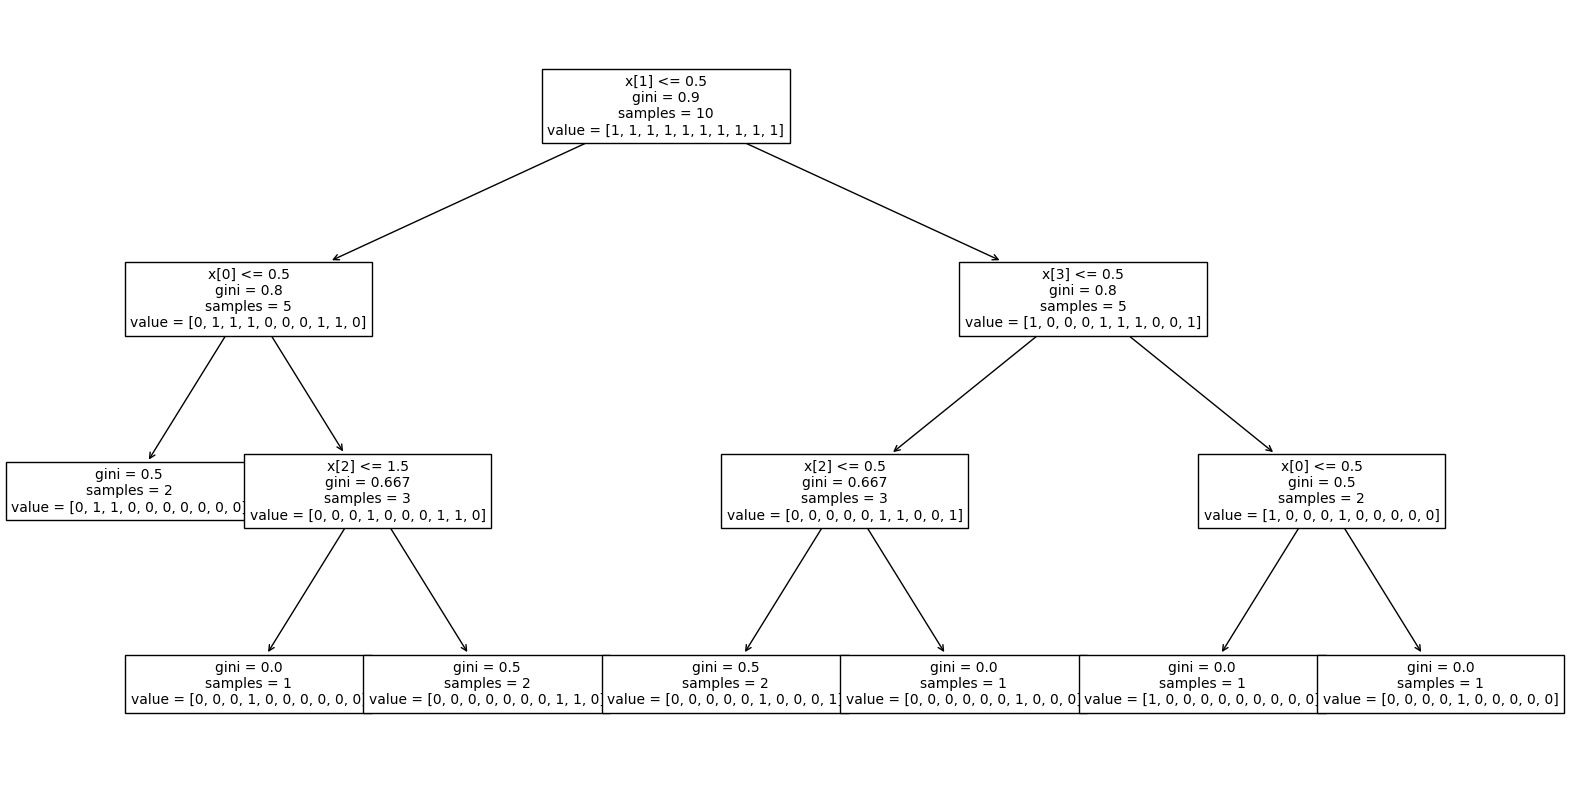
\includegraphics[width = 0.5\textwidth]{output.png}
\end{figure}

\end{enumerate}

\item 
\begin{enumerate}
\item Considering the MLE with \(\mu\)
\[\mu = \arg\max_{\mu} L(\theta)\]

Considering \(\sigma\) as a constant, one can derive
\[\mu = \arg\min \sum_{i = 1}^n(\mu - x_i) = \frac 1 n \sum_{i = 1}^n x_i\]

\item Considering optimize the ML with \(\sigma\), one can derive
\[\sigma = \arg\max_{\sigma} L(\theta)\]

Derivate the formula with variable \(\sigma\), use the notation \(s\) to representate \(\sum_{i = 1}^n (x_i - \mu
)^2\).

One can get 

\[\frac{s - n\sigma^2}{\sigma^{n + 3}} \implies \sigma^2 = \frac s n = \frac{1}{n}\sum_{i = 1}^n (x_i - \mu)^2\]

Use the the MLE  \(\hat\mu\) to replace \(\mu\), one can get the hypothesis.

\item Considering
\begin{align*}
    E(\hat \mu) &= \frac 1 n E(\sum_{i = 1}^n x_i)\\
    &= \frac 1 n \sum_{i = 1}^n E(x_i)\\
    &= \frac 1 n \cdot n\mu = \mu\\
\end{align*}

Considering
\begin{align*}
    E(\hat \sigma^2) &= \frac{1}{n - 1}E([\sum_{i = 1}^n (x_i - \bar x)]^2)\\
\end{align*}

And \((\frac{(x_i - \mu)}{\sigma})^2 \sim \mathcal{X}^2(n)\), thus

\[E = \frac{1}{n - 1}(n - 1)\sigma^2 = \sigma^2\]



\end{enumerate}

\item 
\begin{enumerate}
\item Considering writing the likelihood fuction by \(L(\theta) = P_X P_Y\), thus the MLE of \(p_k\) is equivalent to the MLE of \(P_Y\). And as \(y\) is a discrete variable, one can easily get the rsult as 

\[\hat p_k = \frac{Count(y = k)}{n} = \frac{\sum_{i = 1}^n I(y_i = k)}{n}\]

\item 
Use the MLE of \(p_k\) to estimate the \(p_{sk}\), one can note that 
\[\hat p_{sk} = \frac{Count(x = s | y = k)}{Count(y = k)} = \frac{\sum_{i = 1}^n O(x_i = s, y_i = k)}{\sum_{i = 1}^n I(y_i = k)}\]

\end{enumerate}



\item Considering the probability of \(1-NN\) got a wrong answer, noted it as \(W\). And define \(W_0, W_1\) as Bayes Classifier is wrong and with a prediction 0, 1, alsp \(W\) as the Bayes Classifier is wrong. And \(R_0, R_1\) as Bayes Classifier iw right and with a result 0, 1 repectly. Note the results of two classifiers are different with symbol \(D\).

\begin{align*}
    P(W) & \le P(W | W_0)P(W_0) + P(W | W_1)P(W_1) + P(W | R_0)P(R_1) P(W | R_1)P(R_1)\\
    &\le P(W_0) + P(W_1) + P(W | R_0) + P(W | R_1)\\
    &\le 2 P(W) + P(D)\\
\end{align*}

Then, calculate the expectation in the trainging set, one can derive 
\[E_S \mathcal{E}(f^{1NN}) \le 2 \mathcal E f^* + E_S E_x \|\eta - \eta_\pi\|\]

As the case \(D\) is totally equivalent with the result of the absolute value.

Use the Lipschitz Condition, one can derive the result.


\end{enumerate}
\end{document}